Recall the Construction Problem for rings: given a ring, we'd like to construct new rings out of its ``parts''.
So far we've seen several examples of how this can be done including by generating subrings, taking direct sums, constructing rings of fractions, and using polynomials.
This chapter is devoted to yet another method for building new rings out of old ones -- by constructing \emph{quotients}.
This idea is very frequently a stumbling block for beginning students of mathematics, so we will spend some time on it.
But our effort will be rewarded.
Quotient rings are an extremely powerful and natural idea, and more generally the concept of ``quotient'' used here is pervasive in other branches of math.
In a very specific sense quotient rings are the ``opposites'' of subrings.

Here is the basic idea: given a ring \(R\) and an equivalence relation \(\Phi\) on \(R\), we partition \(R\) into equivalence classes as \(R/\Phi\).
Now we attempt to define an arithmetic on \emph{equivalence classes} as follows.
\begin{enumerate}
\item Given two \(\Phi\)-\emph{classes}, say \(X\) and \(Y\) in \(R/\Phi\), first \textbf{choose} some representatives \(x \in X\) and \(y \in Y\).
Now compute the sum \(x+y\) in \(R\).
This element is in some other \(\Phi\)-class \(Z\) in \(R/\Phi\).
We define \(Z\) to be the sum of \(X\) and \(Y\).
\item Likewise, to multiply classes, we \textbf{choose} representatives, multiply in \(R\), and determine the class of the product.
\end{enumerate}
This is a fine idea, and in fact this is precisely how arithmetic works in \(\ZZ/(n)\).
But unfortunately there is a problem: the sum of two classes may depend on our \textbf{choice} of representatives.
Specifically, choosing one pair of representatives \(v_1\) and \(w_1\) may end up in one class, while another pair \(v_2\) \(w_2\) may end up in another class; see \autoref{fig:quot-bad} for an illustration.
\begin{figure}[h!]
\begin{center}
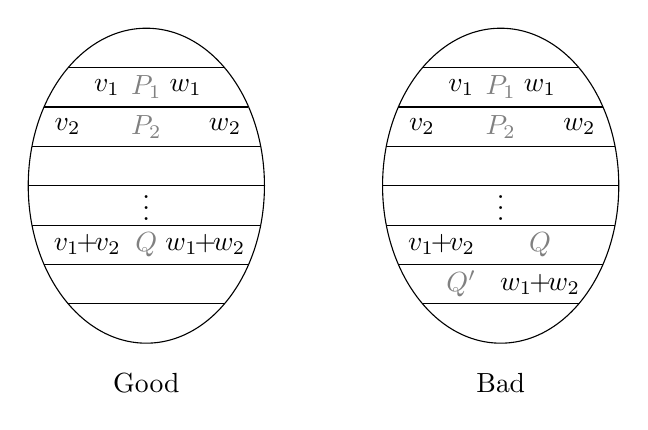
\begin{tikzpicture}[scale=0.5]
  \draw (3,4) ellipse (3 and 4);
  \draw (1.02,1) edge (4.98,1);
  \draw (0.40,2) edge (5.59,2);
  \draw (0.09,3) edge (5.90,3);
  \draw (0.00,4) edge (6.00,4);
  \draw (0.09,5) edge (5.90,5);
  \draw (0.40,6) edge (5.59,6);
  \draw (1.02,7) edge (4.98,7);
  \node at (3,3.65) {\(\vdots\)};
  \node at (2,6.5) {\(v_1\)};
  \node at (4,6.5) {\(w_1\)};
  \node at (1,5.5) {\(v_2\)};
  \node at (5,5.5) {\(w_2\)};
  \node at (1.5,2.5) {\(v_1\!\!+\!\!v_2\)};
  \node at (4.5,2.5) {\(w_1\!\!+\!\!w_2\)};
  \node at (3,6.5) [gray] {\(P_1\)};
  \node at (3,5.5) [gray] {\(P_2\)};
  \node at (3,2.5) [gray] {\(Q\)};
  \node at (3,-1) {Good};
  \draw (12,4) ellipse (3 and 4);
  \draw (10.02,1) edge (13.98,1);
  \draw (09.40,2) edge (14.59,2);
  \draw (09.09,3) edge (14.90,3);
  \draw (09.00,4) edge (15.00,4);
  \draw (09.09,5) edge (14.90,5);
  \draw (09.40,6) edge (14.59,6);
  \draw (10.02,7) edge (13.98,7);
  \node at (12,3.65) {\(\vdots\)};
  \node at (11,6.5) {\(v_1\)};
  \node at (13,6.5) {\(w_1\)};
  \node at (10,5.5) {\(v_2\)};
  \node at (14,5.5) {\(w_2\)};
  \node at (10.5,2.5) {\(v_1\!\!+\!\!v_2\)};
  \node at (13,1.5) {\(w_1\!\!+\!\!w_2\)};
  \node at (12,6.5) [gray] {\(P_1\)};
  \node at (12,5.5) [gray] {\(P_2\)};
  \node at (13,2.5) [gray] {\(Q\)};
  \node at (11,1.5) [gray] {\(Q^\prime\)};
  \node at (12,-1) {Bad};
\end{tikzpicture}
\caption{\label{fig:quot-bad} What can go wrong when making partitions into rings.}
\end{center}
\end{figure}
More concretely we can try this strategy by partitioning the set of integers into two sets; the primes \(P\) and the nonprimes \(N\).
We might try to compute the sum \(P+P\) using representatives \(2\) and \(3\); in this case \[ P + P = [2] + [3] = [2+3] = [5] = P. \]
But if we use representatives \(3\) and \(7\), we have \[ P + P = [3] + [7] = [3+7] = [10] = N. \]
This is a problem -- it means that this \(+\) operation is not well-defined.
To fix the problem, we just need to make sure our partition is chosen so that this bad thing never happens.

\begin{dfn}[Ring Congruence] \label{dfn:ring-congruence}
Let \(R\) be a ring.
An equivalence relation \(\Phi\) on \(R\) is called a \emph{congruence}\index{congruence} if the following hold.
\begin{proplist*}
\item If \(x_1 \mathrel{\Phi} x_2\) and \(y_1 \mathrel{\Phi} y_2\), then \((x_1+y_1) \mathrel{\Phi} (x_2+y_2)\).
\item If \(x_1 \mathrel{\Phi} x_2\) and \(y_1 \mathrel{\Phi} y_2\), then \((x_1 y_1) \mathrel{\Phi} (x_2 y_2)\).
\end{proplist*}
\end{dfn}

So a congruence is a particular kind of equivalence relation.
The congruence condition may at first glance seem to be very strong -- so strong that it is not immediately clear that interesting congruences should even exist.
(We will see that they do, and are abundant).

\begin{examples}
\item Let \(R\) be a ring.
Then the \emph{diagonal} relation \(\Delta = \{ (r,r) \mid r \in R \}\) and the \emph{universal} relation \(\nabla = \{ (r,s) \mid r,s \in R \}\) are both congruences.
These are called the \emph{trivial} congruences on \(R\).

\item The relation \(\Phi\) on \(\ZZ\) defined by \(r \mathrel{\Phi} s \Leftrightarrow n|(s-r)\) is a congruence.
In fact \(\ZZ\) here can be replaced by any commutative ring \(R\) and \(n\) by any fixed element of \(R\).
\end{examples}

\begin{prop}
Let \(R\) be a ring and \(\Phi\) an equivalence on \(R\).
\begin{proplist}
\item The operations \(+\) and \(\cdot\) on \(R/\Phi\) given by \[ [a] + [b] = [a+b] \quad \mathrm{and} \quad [a] \cdot [b] = [a \cdot b] \] are well-defined if and only if \(\Phi\) is a congruence.
\item In this case, \((R/\Phi, +, \cdot)\) is a ring, called the \emph{quotient} of \(R\) by \(\Phi\).
If \(R\) is commutative, then \(R/\Phi\) is commutative, and if \(R\) is unital, the \(R/\Phi\) is unital.
\end{proplist}
\end{prop}

\begin{proof}
\begin{inlineproplist}
\item If we want to be pedantic (and we do!), the precise operations on \(R/\Phi\) are \[ \mathsf{plus} = \left\{ \left(([a],[b]), [a+b]\right) \mid a,b \in R \right\} \] and \[ \mathsf{times} = \left\{ \left(([a],[b]), [ab]\right) \mid a,b \in R \right\}. \]
First, suppose \(\Phi\) is a congruence, and suppose we have elements \((([a_1],[b_1]),[a_1+b_1])\) and \((([a_2],[b_2]),[a_2+b_2])\) in \(\mathsf{plus}\) such that \([a_1] = [a_2]\) and \([b_1] = [b_2]\).
Then (by definition) \(a_1 \mathrel{\Phi} a_2\) and \(b_1 \mathrel{\Phi} b_2\).
Since \(\Phi\) is a congruence, \(a_1 + b_1 \mathrel{\Phi} a_2 + b_2\), and thus \([a_1 + b_1] = [a_2 + b_2]\); so \(\mathsf{plus}\) is well-defined.
A similar argument shows that \(\mathsf{times}\) is well-defined.
Conversely, suppose \(\mathsf{plus}\) and \(\mathsf{times}\) are well-defined.
If \(a_1 \mathrel{\Phi} a_2\) and \(b_1 \mathrel{\Phi} b_2\), then \([a_1] = [a_2]\) and \([b_1] = [b_2]\), so that \([a_1+b_1] = [a_1] + [b_1] = [a_2] + [b_2] = [a_2+b_2]\), and thus \(a_1+b_1 \mathrel{\Phi} a_2+b_2\).
Similarly we can show that \(a_1b_1 \mathrel{\Phi} a_2b_2\) so that \(\Phi\) is a congruence.
\item Showing that all 6 of the ring axioms is somewhat tedious; for instance, to show A1 note that if \(a,b,c \in R\), we have \[ ([a] + [b]) + [c] = [a+b] + [c] = [(a+b)+c] = [a+(b+c)] = [a] + [b+c] = [a] + ([b] + [c]). \]
Similarly if \(R\) is commutative then \( [a][b] = [ab] = [ba] = [b][a] \) for all \(a,b \in R\).
Finally, if \(R\) is unital, then evidently \([1_R]\) is a one in \(R/\Phi\).
\end{inlineproplist}
\end{proof}

Quotients are thus -- potentially -- a rich new source of examples of rings.
There are some potential problems, however.
First, it is not immediately clear how we can find interesting congruences.
Second, once we have a congruence, it is not clear how we can effectively detect when two elements of \(R\) are in the same \(\Phi\)-class.
This means that even detecting when two elements of \(R/\Phi\) are equal may be difficult -- which has important computational consequences.
Third, since quotient rings are sets of sets, the most natural way to define a mapping on \(R/\Phi\), in terms of class representatives, is fraught with danger.
We expect that finding well-defined homomorphisms from a quotient ring will be difficult.
Fortunately we will see that all three of these problems have nice resolutions.

As an example, what can we say about the ring \(\QQ[x]/(x^2 + 1)\)?
Using the division algorithm, every polynomial in \(\QQ[x]\) can be written as \((x^2+1)q(x) + r(x)\), where \(r\) is either 0, a nonzero constant, or a linear polynomial. Etc. etc.



%---------%
\Exercises%
%---------%

\begin{exercise}
Let \(R\) be a ring, and let \(\Delta\) and \(\nabla\) denote the trivial and universal congruences on \(R\).
Show that \(R \cong R/\Delta\) and \(0 \cong R/\nabla\).
\end{exercise}


\begin{exercise}
(One-sided ideals)
\end{exercise}
